% ---------------------------------------------------------------- Method validation: offline results
\subsection*{Offline results}
Table~\ref{tab:main} lists every policy under both protocols, and Fig.~\ref{fig:frontier} places the learned gates and the patience rule on the trade-off between compute saved and regret. Four observations follow.

\paragraph{The gate transfers to unseen workloads} Trained on three workloads and applied to the fourth, the KAN gate saved \R{lowo}{kan}{saved}\% of all epochs (95\% CI \R{lowo}{kan}{savedlo} to \R{lowo}{kan}{savedhi}) at a mean regret of \R{lowo}{kan}{regret}\% (CI \R{lowo}{kan}{regretlo} to \R{lowo}{kan}{regrethi}), with \R{lowo}{kan}{prem}\% of runs stopped prematurely and a mean accuracy loss of \R{lowo}{kan}{acc} percentage points. Within a workload it saved \R{within}{kan}{saved}\% at \R{within}{kan}{regret}\% regret with \R{within}{kan}{prem}\% premature stops, so moving to an unseen workload cost no quality and about two percentage points of savings. Transfer works because every feature is normalised per run: a gate learns what a plateau looks like, not the loss level of a particular dataset. Of all learned gates, the KAN had the lowest mean regret and premature-stop rate under transfer (Table~\ref{tab:main}); the MLP and the depth-3 tree saved more compute but stopped \R{lowo}{mlp}{prem}\% and \R{lowo}{tree}{prem}\% of runs prematurely, and their regret was significantly higher ($p\T{lowo}{mlp}{regret}{p}$ and $p\T{lowo}{tree}{regret}{p}$, Table~\ref{tab:tests}).

\paragraph{Hindsight labels are what make the gate useful} The same KAN, trained on the same real decision points but with the labels of the hand-written rule, saved only \R{lowo}{kanrule}{saved}\% under transfer (\R{within}{kanrule}{saved}\% within workloads) and stopped runs significantly later ($p\T{lowo}{kanrule}{stop}{p}$), with no significant difference in regret ($p\T{lowo}{kanrule}{regret}{p}$). The rule itself, applied directly, stopped \R{lowo}{rule}{prem}\% of runs prematurely. Imitating a rule therefore produces a cautious copy of the rule's thresholds, while hindsight labels produce a gate that stops when the remaining improvement is actually small.

\paragraph{A well-chosen patience rule is as good on the stopping axis} Patience 8 saved \R{lowo}{pateight}{saved}\% at \R{lowo}{pateight}{regret}\% regret, and the regret of the KAN gate is not significantly different from it ($p\T{lowo}{pateight}{regret}{p}$); patience stopped slightly earlier ($p\T{lowo}{pateight}{stop}{p}$). On the frontier of Fig.~\ref{fig:frontier} the patience family and the linear gate lie at or slightly above the KAN gate's curve, i.e.\ for the stop decision alone they reach the same regret with a few percentage points more compute saved. Shorter patience is clearly worse: patience 3 stopped \R{lowo}{patthree}{prem}\% of runs prematurely. The median stopping rule had a mean regret of \R{lowo}{median}{regret}\%, because in a grid of learning rates it stops slow-starting configurations that later become the best; it is designed for comparing trials, not for deciding when a single job has finished. The value of the KAN gate is therefore not a better stopping trade-off than a tuned patience rule. It is that a single learned rule, with no per-workload tuning, makes calibrated stop decisions on unseen workloads, also decides when to adjust the learning rate, and is an explicit formula whose every decision can be recomputed and attributed.

\paragraph{Every workload behaves consistently} Table~\ref{tab:perworkload} breaks the transfer result down by held-out workload. The KAN gate kept mean regret at or below 0.6\% on every held-out workload, including CIFAR-10, the only colour-image workload, and the SGD-trained MLP, the only workload with a different optimiser. Its largest single-run regret, \R{lowo}{kan}{max}\%, occurs on one unstable SGD run (learning rate 0.3) whose validation loss hovers without progress for about 15 epochs and then reaches its best value in a single isolated dip at epoch 21; every hindsight-trained gate and both patience 5 and patience 8 stop that run before the dip, and only the oracle does not.

\begin{table}[p]
\centering
\caption{Offline replay on \nRuns{} real runs. Compute saved and mean regret with 95\% bootstrap confidence intervals; ``prem.'' is the share of runs stopped with more than 2\% regret. Within: seed-grouped 3-fold cross-validation inside each workload. LOWO: trained on three workloads, tested on the fourth. Policies without training (patience, median rule, rule, oracle, no stopping) are identical under both protocols.}
\label{tab:main}
\footnotesize
\setlength{\tabcolsep}{3.5pt}
\resizebox{\textwidth}{!}{%
\begin{tabular}{lrrrrrr}
\toprule
& \multicolumn{3}{c}{Within-workload} & \multicolumn{3}{c}{Leave-one-workload-out} \\
\cmidrule(lr){2-4}\cmidrule(lr){5-7}
Policy & Saved (\%) & Regret (\%) & Prem.\ (\%) & Saved (\%) & Regret (\%) & Prem.\ (\%) \\
\midrule
\tabinput{generated/table_main.tex}
\bottomrule
\end{tabular}}
\end{table}

\begin{figure}[p]
\centering
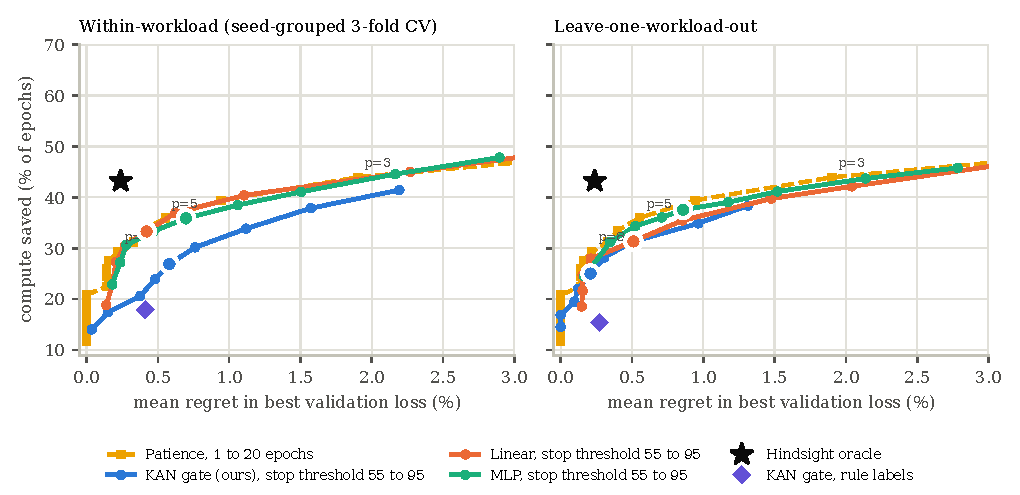
\includegraphics[width=\textwidth]{figures/frontier.pdf}
\caption{Trade-off between compute saved and mean regret. Learned gates are traced by sweeping the stop threshold from 55 to 95 (large dot: the deployed threshold 75); the dashed line is the patience rule for patience 1 to 20 epochs. Points further up and to the left are better. The median stopping rule (mean regret \R{lowo}{median}{regret}\%) lies outside the plotted range.}
\label{fig:frontier}
\end{figure}

\begin{table}[t]
\centering
\caption{Leave-one-workload-out results per held-out workload: compute saved (\%) / mean regret (\%).}
\label{tab:perworkload}
\footnotesize
\resizebox{\textwidth}{!}{%
\begin{tabular}{lcccc}
\toprule
Policy & Fashion-MNIST CNN & MNIST CNN & CIFAR-10 CNN & F-MNIST MLP (SGD) \\
\midrule
\tabinput{generated/table_per_workload.tex}
\bottomrule
\end{tabular}}
\end{table}

\begin{table}[t]
\centering
\caption{Paired comparison of the KAN gate with each alternative over \nRuns{} runs: median difference (KAN minus alternative) in stop epoch and in regret (percentage points), with Holm-corrected Wilcoxon signed-rank $p$-values. A negative stop difference means the KAN gate stops earlier.}
\label{tab:tests}
\footnotesize
\setlength{\tabcolsep}{4pt}
\resizebox{\textwidth}{!}{%
\begin{tabular}{lrrrrrrrr}
\toprule
& \multicolumn{4}{c}{Within-workload} & \multicolumn{4}{c}{Leave-one-workload-out} \\
\cmidrule(lr){2-5}\cmidrule(lr){6-9}
Alternative & $\Delta$stop & $p$ & $\Delta$regret & $p$ & $\Delta$stop & $p$ & $\Delta$regret & $p$ \\
\midrule
\tabinput{generated/table_tests.tex}
\bottomrule
\end{tabular}}
\end{table}

\subsection*{Ablations}
Table~\ref{tab:ablation} repeats the leave-one-workload-out evaluation with one feature at a time replaced by its training mean, and with three hindsight tolerances. Epochs since improvement ($x_5$) carries most of the decision: without it the gate stops much earlier and regret rises from \A{none}{regret}\% to \A{x5}{regret}\%. The plateau score ($x_1$) and the oscillation feature ($x_3$) each add a few percentage points of compute saved at unchanged regret; gradient trend ($x_2$) and budget remaining ($x_4$) change little on these workloads. The tolerance $\tau$ is a direct and predictable control of the trade-off: $\tau=2\%$ gives \Sw{2}{saved}\% saved at \Sw{2}{regret}\% regret and $\tau=10\%$ gives \Sw{10}{saved}\% at \Sw{10}{regret}\%, so an operator sets the acceptable loss of quality in the units in which it is measured.

\begin{table}[t]
\centering
\caption{Feature ablation and tolerance sweep, leave-one-workload-out, KAN gate (three gate seeds). Top: one feature replaced by its training-set mean in training and test. Bottom: hindsight tolerance $\tau$ (default 5\%).}
\label{tab:ablation}
\small
\begin{tabular}{lrrr}
\toprule
Feature removed / setting & Saved (\%) & Regret (\%) & Premature (\%) \\
\midrule
\tabinput{generated/table_ablation.tex}
\bottomrule
\end{tabular}
\end{table}
